% Unofficial University of Cambridge Poster Template
% https://github.com/andiac/gemini-cam
% a fork of https://github.com/anishathalye/gemini
% also refer to https://github.com/k4rtik/uchicago-poster

\documentclass[final]{beamer}

% ====================
% Packages
% ====================

\usepackage[T1]{fontenc}
\usepackage{lmodern}
\usepackage[size=custom,width=120,height=72,scale=1.0]{beamerposter}
\usetheme{gemini}
\usecolortheme{cam}
\usepackage{graphicx}
\usepackage{booktabs}
\usepackage{tikz}
\usepackage{pgfplots}
\pgfplotsset{compat=1.14}
\usepackage{anyfontsize}

% ====================
% Lengths
% ====================

% If you have N columns, choose \sepwidth and \colwidth such that
% (N+1)*\sepwidth + N*\colwidth = \paperwidth
\newlength{\sepwidth}
\newlength{\colwidth}
\setlength{\sepwidth}{0.025\paperwidth}
\setlength{\colwidth}{0.3\paperwidth}
\setlength{\paperwidth}{48in}
\setlength{\paperheight}{36in}
\newcommand{\separatorcolumn}{\begin{column}{\sepwidth}\end{column}}

% ====================
% Title
% ====================

\title{Discover User-App Interactions \& \\  
Solutions to Reducing the Initial User-CPU Latency
}

\author{Thy Nguyen \and Milon Chakkalakal \and Pranav Thaenraj}

\institute[shortinst]{Advisors: Jamel Tayeb, Bijan Arbab, Sruti Sahani, Oumaima Makhlouk, Praveen Polasam, Chansik Im}

% ====================
% Footer (optional)
% ====================

\footercontent{
  \href{https://www.example.com}{https://www.example.com} \hfill
  ABC Conference 2025, New York --- XYZ-1234 \hfill
  \href{mailto:alyssa.p.hacker@example.com}{alyssa.p.hacker@example.com}}
% (can be left out to remove footer)

% ====================
% Logo (optional)
% ====================

% use this to include logos on the left and/or right side of the header:
% \logoright{\includegraphics[height=7cm]{logo1.pdf}}
% \logoleft{\includegraphics[height=7cm]{logo2.pdf}}

% ====================
% Body
% ====================

\begin{document}

% Refer to https://github.com/k4rtik/uchicago-poster
% logo: https://www.cam.ac.uk/brand-resources/about-the-logo/logo-downloads
\addtobeamertemplate{headline}{}
{
    \begin{tikzpicture}[remember picture,overlay]
      \node [anchor=north west, inner sep=3cm] at ([xshift=0.0cm,yshift=0.75cm]current page.north west)
      {
\includegraphics[height=5.5cm]{HDSI_Intel.png}}; 
    \end{tikzpicture}

    \begin{tikzpicture}[remember picture,overlay]
      \node [anchor=north west, inner sep=3cm] at ([xshift=110.0cm,yshift=0.75cm]current page.north west)
      {
\includegraphics[height=5.5cm]{ucsd_logo.png}}; 
    \end{tikzpicture}
}

\begin{frame}[t]
\begin{columns}[t]
\separatorcolumn

\begin{column}{\colwidth}

  \begin{block}{Abstract}

    Some block contents, followed by a diagram, followed by a dummy paragraph.

    Lorem ipsum dolor sit amet, consectetur adipiscing elit. Morbi ultricies
    eget libero ac ullamcorper. Integer et euismod ante. Aenean vestibulum
    lobortis augue, ut lobortis turpis rhoncus sed. Proin feugiat nibh a
    lacinia dignissim. Proin scelerisque, risus eget tempor fermentum, ex
    turpis condimentum urna, quis malesuada sapien arcu eu purus.

  \end{block}

    \begin{alertblock}{Methodology of Data Collection}

    We write the \textbf{\textit{input libraries (ILs)}} using the  software development kit \textbf{\textit{XLSDK User Guide}}, along with the \textbf{\textit{Environment Server (ESRV)}}  toolchain  and the \textit{ \textbf{Intel® System Usage Report  (SUR)}} framework to anonymously gather and analyze data usage from multiple devices. The ILs include: 

    \begin{itemize}
      \item \textbf{Mouse Input IL}  to capture the (X, Y) positions of the mouse in pixels (with or without noise)

      \item \textbf{User Wait IL} to retrieve the cursor type (e.g. loading or working smoothly) and its timestamp 

      \item \textbf{Mouse Hook IL} to track the UI objects clicked by the mouse

      \item \textbf{Foreground Window IL} to log the window's details detected by mouse clicks or time ticks

      \item \textbf{Desktop Mapper IL} to map all the open app windows in the z-order and store the relative position of an app on the screen as well as their individual size

    \end{itemize}

    We mainly focus on the data collected from the \textit{Foreground Window IL} for further exploration.
    \begin{figure}
      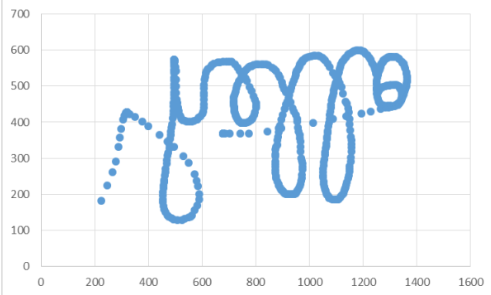
\includegraphics[width=0.475 \textwidth, height=11.5cm]{mouse_movement.png}
        \hspace{\fill}
        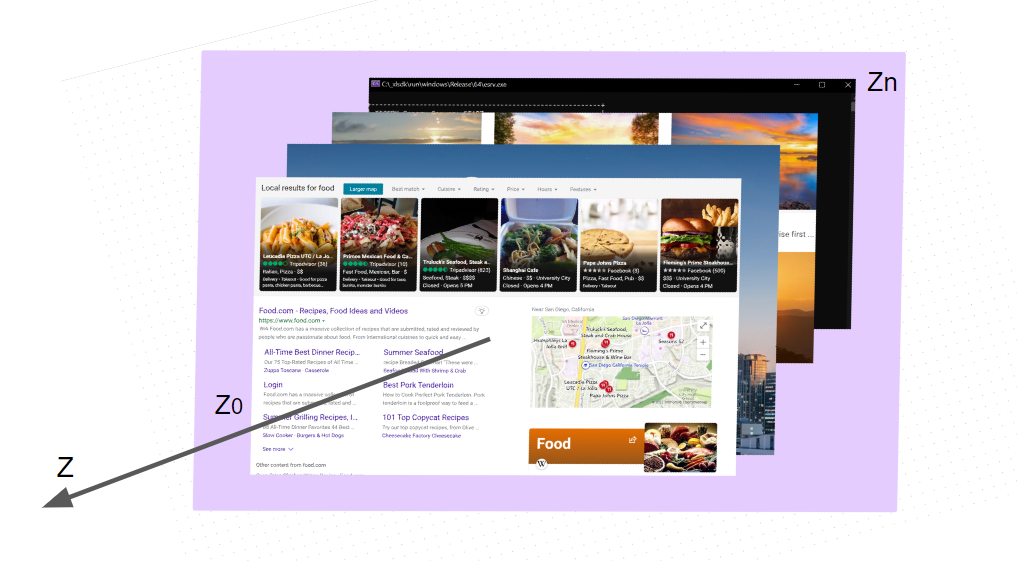
\includegraphics[width=0.475\textwidth, height=11.5cm]{foreground_desktopMapper.PNG}
      \caption{Mouse Movement, Foreground Window, and Z-axis}\label{fig:xyz}
    \end{figure}
  \end{alertblock}

  \begin{block}{Data Preprocessing}
  \end{block}
\begin{block}{Exploratory Data Analysis}

    Et rutrum ex euismod vel. Pellentesque ultricies, velit in fermentum
    vestibulum, lectus nisi pretium nibh, sit amet aliquam lectus augue vel
    velit. Suspendisse rhoncus massa porttitor augue feugiat molestie. Sed
    molestie ut orci nec malesuada. Sed ultricies feugiat est fringilla
    posuere.

    \begin{figure}
      \centering
      \begin{tikzpicture}
        \begin{axis}[
            scale only axis,
            no markers,
            domain=0:2*pi,
            samples=100,
            axis lines=center,
            axis line style={-},
            ticks=none]
          \addplot[red] {sin(deg(x))};
          \addplot[blue] {cos(deg(x))};
        \end{axis}
      \end{tikzpicture}
      \caption{Another figure caption.}
    \end{figure}
    \begin{figure}
      \centering
      \begin{tikzpicture}[scale=6]
        \draw[step=0.25cm,color=gray] (-1,-1) grid (1,1);
        \draw (1,0) -- (0.2,0.2) -- (0,1) -- (-0.2,0.2) -- (-1,0)
          -- (-0.2,-0.2) -- (0,-1) -- (0.2,-0.2) -- cycle;
      \end{tikzpicture}
      \caption{A figure caption.}
    \end{figure}
    \begin{enumerate}
      \item \textbf{Morbi mauris purus}, egestas at vehicula et, convallis
        accumsan orci. Orci varius natoque penatibus et magnis dis parturient
        montes, nascetur ridiculus mus.
      \item \textbf{Cras vehicula blandit urna ut maximus}. Aliquam blandit nec
        massa ac sollicitudin. Curabitur cursus, metus nec imperdiet bibendum,
        velit lectus faucibus dolor, quis gravida metus mauris gravida turpis.
      \item \textbf{Vestibulum et massa diam}. Phasellus fermentum augue non
        nulla accumsan, non rhoncus lectus condimentum.
    \end{enumerate}

  \end{block}

\end{column}

\separatorcolumn

\begin{column}{\colwidth}

\begin{exampleblock}{Methodology of Predictive Tasks}

    \heading{Hidden Markov Model  (HMM)}

   \begin{itemize}
       \item \textbf{Problem Statement}: Predict the likelihood of using an app \textit{given} the former sequence of application usage
       \item \textbf{Basic Idea}: Utilize the conditional probability $P(A|B) = \frac{P(A\cap B)}{P(B)}$
       \item \textbf{HMM Assumptions}:
           
            1. \textbf{Markov Chain} Only the \underline{\textit{current}} state plays the most crucial role in predicting the future in the sequence; other states before that will not influence the future states 

            $$P(q_i = a | q_1q_2...q_{i-1}) = P(q_i= a | q_{i-1})$$

            where $q_k$ are the states for $k \in \{1, 2, ..., i\}$, e.g. hidden states \textit{chrome.exe} and \textit{explorer.exe}

           2. \textbf{Output Independence} The probability of observing an event $o_i$ only relies on the state $q_i$ that \underline{\textit{directly}} produced $o_i$. 
           
           $$P(o_i | q_1, ... q_i , ..., q_T, o_1, ..., o_i, ..., o_T) = P(o_i | q_i)$$
           
           where $o_1o_2...o_T$ is a sequence of T observations and $q_1, q_2 , ...,q_T$ are T states

        \item \textbf{Transition Matrix}:

        \item \textbf{Emission Matrix}: contains the emission probabilities, i.e. the likelihood of moving from one executable file to another app/tab. 
        
        \centering{$P($"chrome.exe" -> "Spotify"$)$ =  $P($"Spotify" | "chrome.exe"$)$}
       \end{itemize}
          
    \heading{Recurrent Neural Network (RNN)}

    \begin{itemize}
       \item \textbf{Problem Statement}: Predict the (total) time usage of an app/tab/recorded process using the past \textit{time-series} data
       \begin{figure}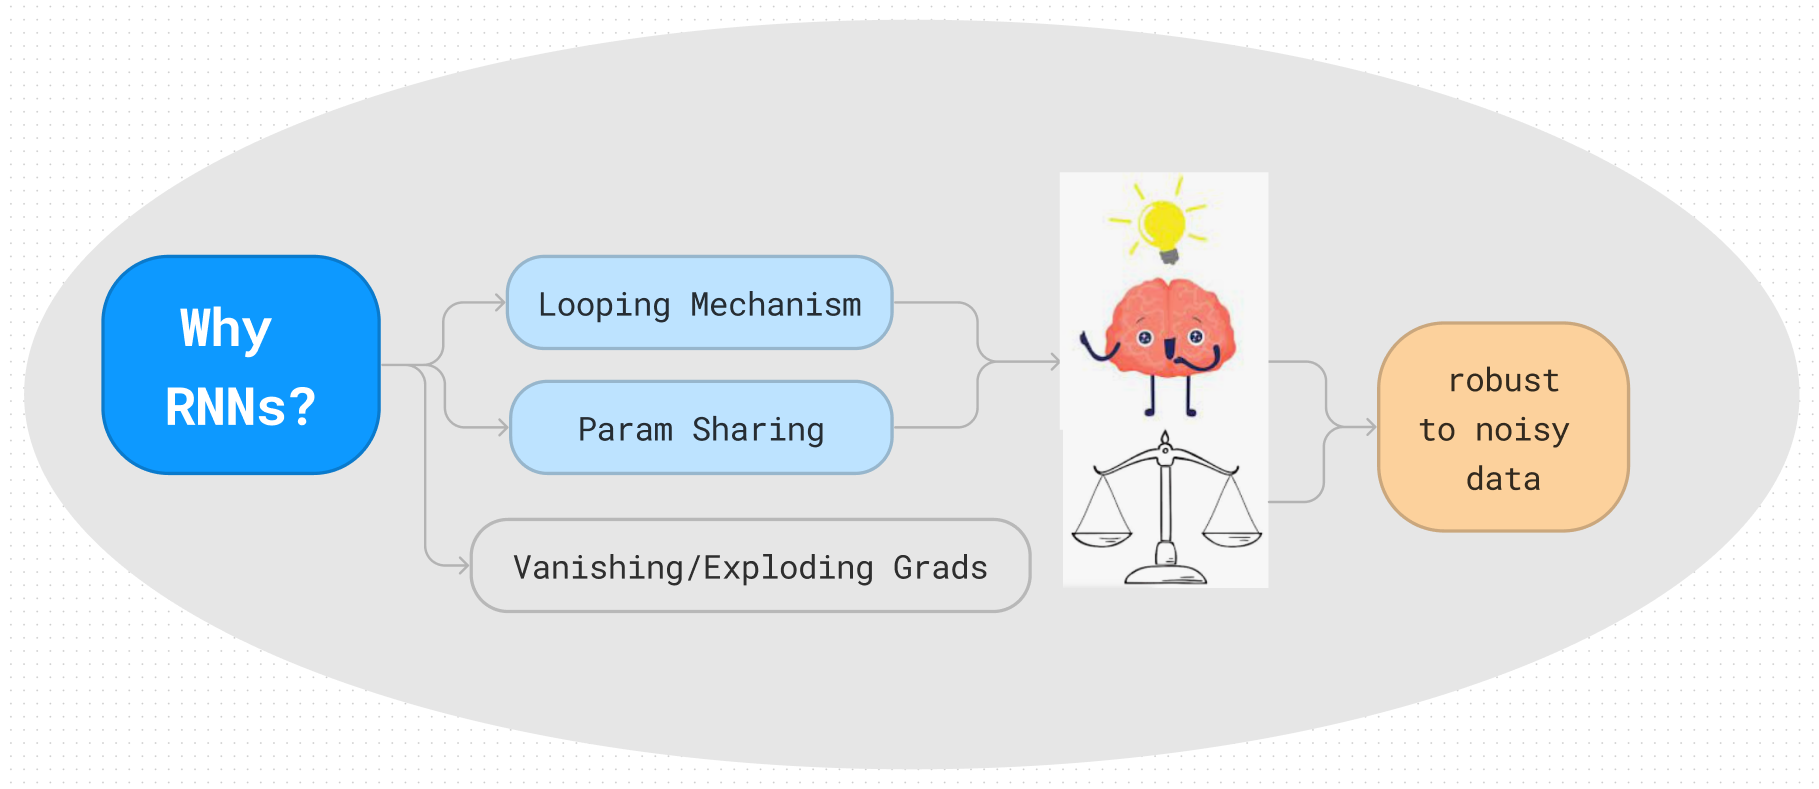
\includegraphics[width=0.8\textwidth, height=12cm]{Why_RNN.PNG}\end{figure}

       \item \textbf{Feature Engineering}:
       
       1. \textbf{Example 1}:

       2. \textbf{Example 2}:
       
       3. \textbf{Example}:
       
       \item \textbf{Experiments with RNNs}:
       
       1. \textbf{Vanilla RNN}: 

       2. \textbf{LSTM}:
       
       3. \textbf{GRU}:




      \end{itemize}
    \end{exampleblock}

    \begin{block}{Prediction Results}

    Class aptent taciti sociosqu ad litora torquent per conubia nostra, per
    inceptos himenaeos. Phasellus libero enim, gravida sed erat sit amet,
    scelerisque congue diam. Fusce dapibus dui ut augue pulvinar iaculis.

    \begin{table}
      \centering
      \begin{tabular}{l r r c}
        \toprule
        \textbf{First column} & \textbf{Second column} & \textbf{Third column} & \textbf{Fourth} \\
        \midrule
        Foo & 13.37 & 384,394 & $\alpha$ \\
        Bar & 2.17 & 1,392 & $\beta$ \\
        Baz & 3.14 & 83,742 & $\delta$ \\
        Qux & 7.59 & 974 & $\gamma$ \\
        \bottomrule
      \end{tabular}
      \caption{A table caption.}
    \end{table}

    Donec quis posuere ligula. Nunc feugiat elit a mi malesuada consequat. Sed
    imperdiet augue ac nibh aliquet tristique. Aenean eu tortor vulputate,
    eleifend lorem in, dictum urna. Proin auctor ante in augue tincidunt
    tempor. Proin pellentesque vulputate odio, ac gravida nulla posuere
    efficitur. Aenean at velit vel dolor blandit molestie. Mauris laoreet
    commodo quam, non luctus nibh ullamcorper in. Class aptent taciti sociosqu
    ad litora torquent per conubia nostra, per inceptos himenaeos.

    Nulla varius finibus volutpat. Mauris molestie lorem tincidunt, iaculis
    libero at, gravida ante. Phasellus at felis eu neque suscipit suscipit.
    Integer ullamcorper, dui nec pretium ornare, urna dolor consequat libero,
    in feugiat elit lorem euismod lacus. Pellentesque sit amet dolor mollis,
    auctor urna non, tempus sem.
\begin{table}
      \centering
      \begin{tabular}{l r r c}
        \toprule
        \textbf{First column} & \textbf{Second column} & \textbf{Third column} & \textbf{Fourth} \\
        \midrule
        Foo & 13.37 & 384,394 & $\alpha$ \\
        Bar & 2.17 & 1,392 & $\beta$ \\
        Baz & 3.14 & 83,742 & $\delta$ \\
        Qux & 7.59 & 974 & $\gamma$ \\
        \bottomrule
      \end{tabular}
      \caption{A table caption.}
    \end{table}
  \end{block}

  

\end{column}

\separatorcolumn

\begin{column}{\colwidth}

  \begin{block}{}

    Class aptent taciti sociosqu ad litora torquent per conubia nostra, per
    inceptos himenaeos. Phasellus libero enim, gravida sed erat sit amet,
    scelerisque congue diam. Fusce dapibus dui ut augue pulvinar iaculis.


    Donec quis posuere ligula. Nunc feugiat elit a mi malesuada consequat. Sed
    imperdiet augue ac nibh aliquet tristique. Aenean eu tortor vulputate,
    eleifend lorem in, dictum urna. Proin auctor ante in augue tincidunt
    tempor. Proin pellentesque vulputate odio, ac gravida nulla posuere
    efficitur. Aenean at velit vel dolor blandit molestie. Mauris laoreet
    commodo quam, non luctus nibh ullamcorper in. Class aptent taciti sociosqu
    ad litora torquent per conubia nostra, per inceptos himenaeos.

    Nulla varius finibus volutpat. Mauris molestie lorem tincidunt, iaculis
    libero at, gravida ante. Phasellus at felis eu neque suscipit suscipit.
    Integer ullamcorper, dui nec pretium ornare, urna dolor consequat libero,
    in feugiat elit lorem euismod lacus. Pellentesque sit amet dolor mollis,
    auctor urna non, tempus sem.

  \end{block}
  
\begin{block}{Conclusion}

    Nulla eget sem quam. Ut aliquam volutpat nisi vestibulum convallis. Nunc a
    lectus et eros facilisis hendrerit eu non urna. Interdum et malesuada fames
    ac ante \textit{ipsum primis} in faucibus. Etiam sit amet velit eget sem
    euismod tristique. Praesent enim erat, porta vel mattis sed, pharetra sed
    ipsum. Morbi commodo condimentum massa, \textit{tempus venenatis} massa
    hendrerit quis. Maecenas sed porta est. Praesent mollis interdum lectus,
    sit amet sollicitudin risus tincidunt non.

    Etiam sit amet tempus lorem, aliquet condimentum velit. Donec et nibh
    consequat, sagittis ex eget, dictum orci. Etiam quis semper ante. Ut eu
    mauris purus. Proin nec consectetur ligula. Mauris pretium molestie
    ullamcorper. Integer nisi neque, aliquet et odio non, sagittis porta justo.

    \begin{itemize}
      \item \textbf{Sed consequat} id ante vel efficitur. Praesent congue massa
        sed est scelerisque, elementum mollis augue iaculis.
        \begin{itemize}
          \item In sed est finibus, vulputate
            nunc gravida, pulvinar lorem. In maximus nunc dolor, sed auctor eros
            porttitor quis.
          \item Fusce ornare dignissim nisi. Nam sit amet risus vel lacus
            tempor tincidunt eu a arcu.
          \item Donec rhoncus vestibulum erat, quis aliquam leo
            gravida egestas.
        \end{itemize}
      \item \textbf{Sed luctus, elit sit amet} dictum maximus, diam dolor
        faucibus purus, sed lobortis justo erat id turpis.
      \item \textbf{Pellentesque facilisis dolor in leo} bibendum congue.
        Maecenas congue finibus justo, vitae eleifend urna facilisis at.
    \end{itemize}
    Etiam sit amet tempus lorem, aliquet condimentum velit. Donec et nibh
    consequat, sagittis ex eget, dictum orci. Etiam quis semper ante. Ut eu
    mauris purus. Proin nec consectetur ligula. Mauris pretium molestie
    ullamcorper. Integer nisi neque, aliquet et odio non, sagittis porta justo.

  \end{block}

  \begin{block}{Future Directions}
......

  \end{block}

  
  \begin{block}{References}

    \nocite{*}
    \footnotesize{\bibliographystyle{plain}\bibliography{poster}}

  \end{block}

\end{column}

\separatorcolumn
\end{columns}
\end{frame}

\end{document}
